% \documentclass[manuscript,review,anonymous]{acmart} % submission
\documentclass[nonacm]{acmart} % preprint
% \acmConference[]{} % need to include this to suppress addresses footer

\begin{document}

%\title{Design Patterns for Intelligent Musical Instruments: Case Studies in Performance}
% \title{Performing with Flexible and Accessible Intelligent Musical Instruments}
% Developing a Creative Practice with Intelligent Musical Instruments
\title{Opening the Design Space: Performing with Intelligent Musical Instruments}


\author{Charles Patrick Martin}
\email{charles.martin@anu.edu.au}
\orcid{0000-0001-5683-7529}
\affiliation{%
  \institution{The Australian National University}
  \city{Canberra}
  \state{ACT}
  \country{Australia}
}

\begin{abstract}
% 1. Context: Explain your work's relevance
Machine generation of symbolic music and digital audio are hot topics but there have been relatively few digital musical instruments that integrate generative AI.
% 2. Need: Identify the research gap
Present musical AI tools are not artist centred and do not support experimentation or integrating into musical instruments or practices.
% 3. Task: Explain your unique angle
We introduce an inexpensive generative AI controller based on a single board computer that connects via MIDI to other musical devices.
Our system uses artist-collected datasets and is trained on a regular computer.
% 4. Goal: State your paper's focus
We aim to demonstrate that our system can open the design space for AI-enabled musical instruments to be created and explored through artistic practice.
% 5. Findings:  Present key results
We contribute four examples of instruments created through a first-person artistic research process and tested in performances.
% 6. Conclusion:  Summarize main takeaway
These examples show our system is feasible, flexible, and musically useful.
% 7. Contribution: Connect to broader impact
Our work could enable artists to explore new interaction and performance schemes with intelligent musical instruments.
\end{abstract}

\keywords{generative AI, small data, human-AI interaction, intelligent musical instruments}

\begin{CCSXML}
<ccs2012>
   <concept>
       <concept_id>10010405.10010469.10010475</concept_id>
       <concept_desc>Applied computing~Sound and music computing</concept_desc>
       <concept_significance>500</concept_significance>
       </concept>
   <concept>
       <concept_id>10003120.10003121</concept_id>
       <concept_desc>Human-centered computing~Human computer interaction (HCI)</concept_desc>
       <concept_significance>500</concept_significance>
       </concept>
   <concept>
       <concept_id>10010147.10010257.10010293.10010294</concept_id>
       <concept_desc>Computing methodologies~Neural networks</concept_desc>
       <concept_significance>100</concept_significance>
       </concept>
 </ccs2012>
\end{CCSXML}

\ccsdesc[500]{Applied computing~Sound and music computing}
\ccsdesc[500]{Human-centered computing~Human computer interaction (HCI)}
\ccsdesc[100]{Computing methodologies~Neural networks}

\maketitle

\section{Introduction}\label{intro}

% focus on interaction mappings and performance experiences, not data and training.

\begin{figure}
    \centering
    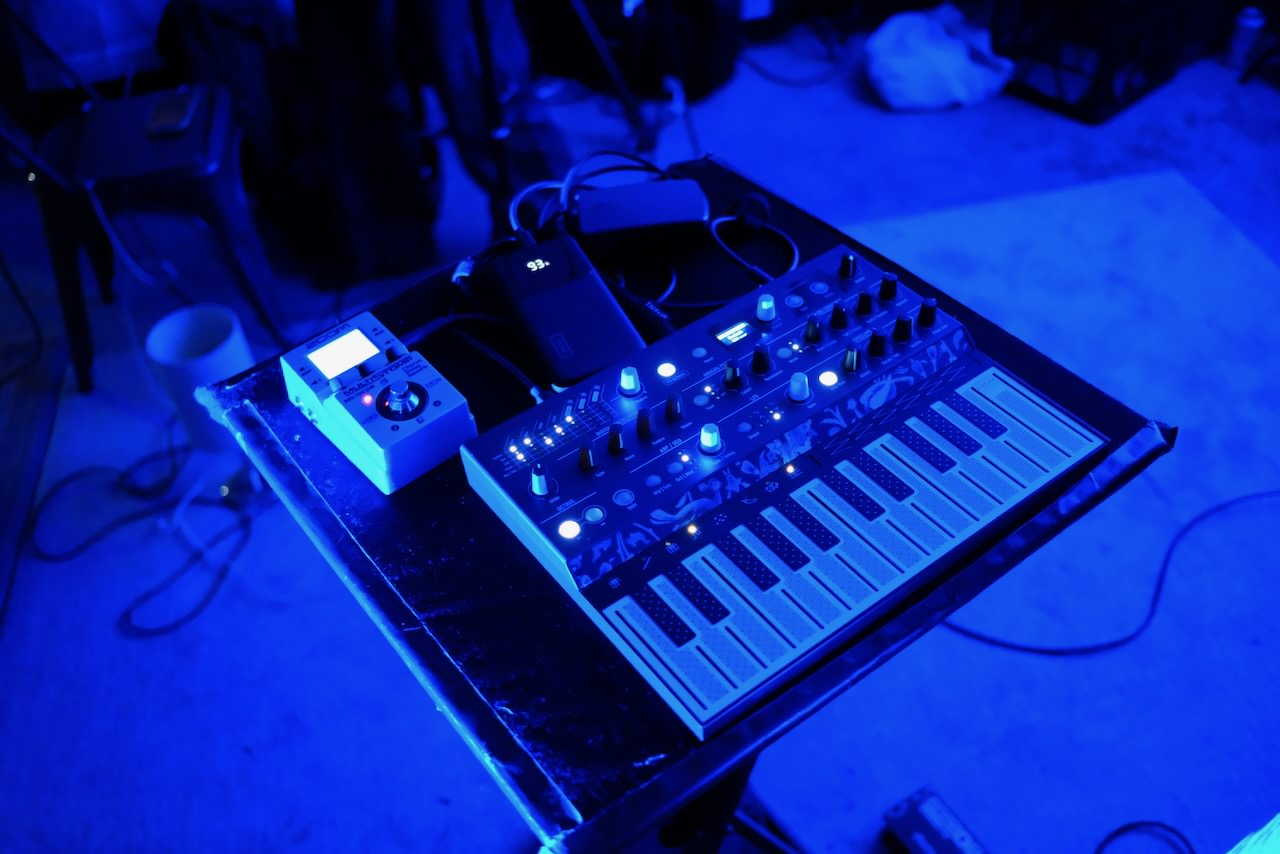
\includegraphics[width=0.49\linewidth]{figures/garage-concert-arturia.jpg}
    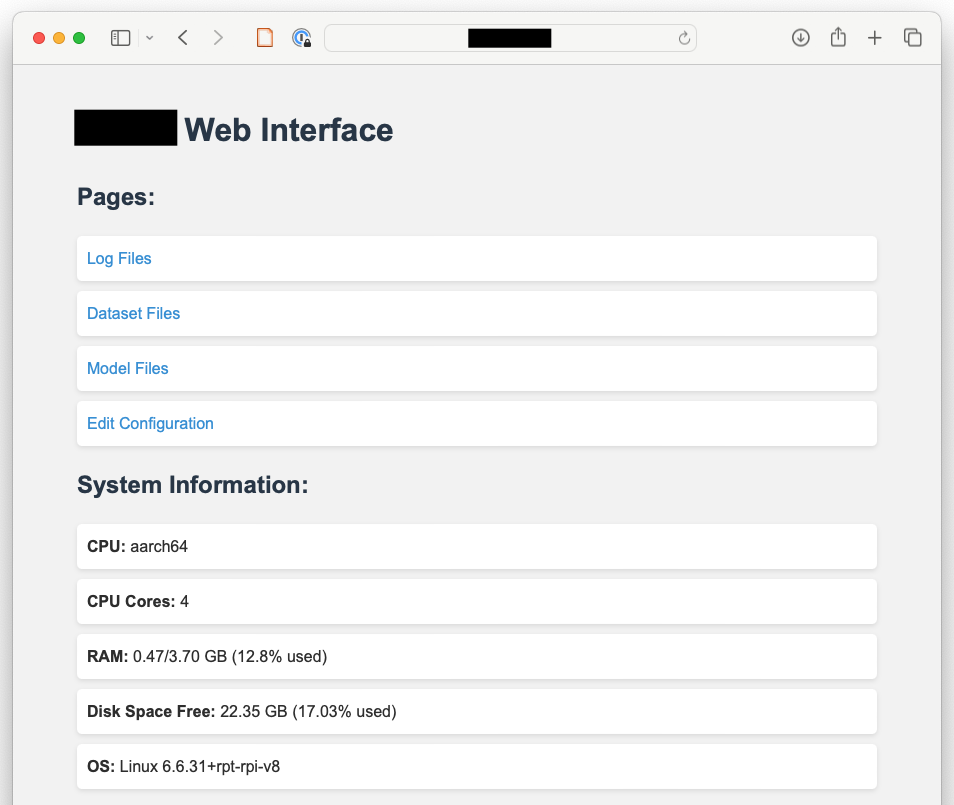
\includegraphics[width=0.39\linewidth]{figures/impsy-web-interface-anon.png}
    \caption{The stage setup for an intelligent musical instrument using our generative AI system running on a Raspberry Pi 4 (left) and the web interface for configuring our system (right). The complete setup of synthesiser, Raspberry Pi, and effects pedal is battery powered. Our software reacts to the musicians' actions through knobs and keys on the synthesiser front panel and controls notes and timbral parameters.}
    \label{fig:int-mus-inst}
\end{figure}

This paper explores how generative AI may be embedded within interactive musical systems for live performance through a series of case study instruments and performances where existing hardware and software instruments have been coupled with a Linux-based single board computer pre-loaded with generative AI software.
A broad range of music technology research has applied AI techniques, and in particular deep learning, for tasks such as mapping, audio or sensor analysis and musical data generation~\cite{jourdan_nime_ml_review}. 
While the analysis of gestures~\cite{visi_iml_gesture} remains a popular application, deep learning models now enable generation of audio~\cite{caillon_rave}, symbolic music~\cite{ji_survey_2024}, and interaction~\cite{Martin2019} data.
Despite this wide range of research, relatively few intelligent musical instruments, that is, digital musical instruments (DMIs) integrating generative AI, are available to be used in ordinary musical practice.
The goal of this research is to open the design space of intelligent musical instruments by introducing a system for creating these instruments that is cheap, small and battery-powered, thus enabling integration into a wider variety of musical systems by a varied population of artists and experimenters. 
Our system includes AI software for generating expressive musical signals from small artist-centred datasets, runs on inexpensive Raspberry Pi computers, and is configurable via a web interface.
As an initial step towards identifying wider variety of intelligent musical instrument designs we report on a series of instruments and performance experiences from a first-person perspective, illustrating different ways that this system can be incorporated into an artistic practice.

AI techniques have been applied in music throughout the history of computing~\cite{roads-music-AI-1985}. Real-time interactive systems became more prominent from the 1990s such as Continuator~\cite{Pachet:2003wd},  Voyager~\cite{Lewis:2000fu}, GenJam~\cite{Biles:2007aa} as well as tools such as Wekinator~\cite{fiebrink_meta-instrument_2009} for embedding machine learning models in new musical systems.
New and more capable deep learning techniques have led to an expansion of interest in AI music making at CHI workshops~\cite{genaichi2022}, music industry white-papers~\cite{goldmedia_ai_2024}, and the general media~\cite{musicpublishers}. Generative AI is now applied in tasks such as sound design~\cite{sound_design_ai_2024}, symbolic music generation~\cite{ji_survey_2024}, and music production~\cite{deruty_development_2022}; however, its use in live musical performances is less widely explored.
With many now framing generative AI as a threat to musicians' livelihoods~\cite{goldmedia_ai_2024} and fraught with ethical pitfalls~\cite{ethical_genaudio_2023}, it may be appropriate to introduce and study artist-centred approaches to creating music with AI.

In this work we introduce a small-data~\cite{Vigliensoni:2022} approach to embedding AI within musical instruments where artists collect, curate, train, and deploy their own intelligent musical instruments.
We define an intelligent musical instrument as an instrument where an AI system generates actions independently of a musician's actions.
This definition would encompass Continuator~\cite{Pachet:2003wd} and Voyager~\cite{Lewis:2000fu} but exclude systems such as Wekinator~\cite{fiebrink_meta-instrument_2009} where AI is only used for mapping musicians' actions or interpreting sensor data.
Our system allows a generative AI algorithm to be incorporated within existing electronic music devices through standard MIDI communication. 
The AI algorithm is able to control not just notes but the significant variety of timbral parameters that are available in electronic instruments. 
Similarly, the AI system can respond to the musician's actions on standard interfaces such as piano-style keyboards as well as other controls such as knobs, sliders, levers, or movement sensors that are typically part of  electronic music devices (e.g., see Figure \ref{fig:int-mus-inst}).
The AI system's interaction mappings are configured through a web interface which is also used to retrieve recorded data for re-training the system's machine learning model.

With our system, intelligent musical instruments can be quickly prototyped and tested through musical performance.
Incorporating generative AI within electronic instruments leverages musicians' existing significant skills and understanding of their instruments which could allow a deeper co-creative practice with an AI system.
In this work, we describe our generative AI music system showing that it is affordable and achievable for non-experts in AI to use.
We document four example intelligent musical instruments and reflections on our continuing practice with this system.
The results contribute an expansion of the design space for intelligent musical instruments, showing that our system is feasible, flexible, and musically useful.
It has been argued that explorations with technology within artistic practices can contribute to HCI~\cite{improvisation-arts-hci-2018, artistic-narratives-hci, state-of-arts-inchi-2022, interactive-art-hci-2019}.
Our work uses artistic methodologies to contribute to the ongoing conversation on design principles and patterns for generative AI in HCI~\cite{design-principles-genai-2024} by examining design possibilities that might encourage more widespread prototyping, hacking, and musicking with AI in musical performance.

% need to more clearly reference main finings.

% need to integrate: feasible, flexible and musically useful
% need to reference HCI and genAI design challenges. Points to make are:
% 1) creative arts is a valid and exciting site for design innovation
% 2) design principles and patterns for generative AI is an ongoing HCI discussion ~\cite{design-principles-genai-2024}

\section{Related Work}\label{related-work}

% \subsection{Generative AI in Performance}

Jourdan and Caramiaux identified gaps in interactivity and practice~\cite{jourdan_nime_ml_review} in AI-supported musical expression, particularly where deep learning is applied. 
They argued that as deep learning systems have become more complex there have been fewer examples of application in long-term musical practice and artists have less interaction with data collection and training phases. 
This contrasts with early AI music systems such as Voyager~\cite{Lewis:2000fu} that were developed over multiple decades and parameter-mapping approaches where long term practice has been studied~\cite{fiebrink_years_ml}.
Tahiroğlu's AI-terity instrument~\cite{tahiroglu-aiterity-2021}, a custom physical interface for exploring AI sound generation while also acting autonomously to engage the performer, has undergone  artist-centred evaluation. 
The experience of performing with AI-terity was later analysed to understand how the system prompted ``unfamiliar musical expectations''~\cite{tahirouglu-evolving-2022}.
This role mirrors some of Parkinson and Dunning's findings for roles that musical machines, including intelligent musical instruments, might have~\cite{taxonomy-music-interactions-parkinson-2025}. They argue that such instruments can ``evolve'', ``collaborate'', and ``learn'' (among other roles). Generative AI may be well placed to help enhance these roles within new musical instruments. 
Generative AI algorithms have also been embedded within software-based instruments. For example, Magenta Studio~\cite{magenta-studio-2019} seeks to embed generative AI algorithms within the Ableton Live digital audio workstation (DAW) software as a plugin that can generate and manipulate MIDI recordings. While these have been examined from an artist perspective~\cite{Davis:2022}, the focus is music production or composition not live performance.

% \subsection{Embedded Musical Instruments}

Incorporating computer music systems into embedded hardware systems can allow better integration into artistic practices with many recent examples using Raspberry Pi~\cite{Berdahl:2013aa} and Beaglebone~\cite{mcpherson-bela-2016} single-board computers. 
Research applying generative AI on such single board computers promises to allow these technologies to be embedded within self-contained musical instruments. 
This has been demonstrated for Raspberry Pi~\cite{Naess:2019aa, martin_empi} and Bela~\cite{pelinski_pipeline_bela} platforms. 
Previous work has acknowledged the difficulties faced by instruments builders wishing to embed AI within new instruments in terms of data collection and training~\cite{Martin2019} and cross-compiling code~\cite{pelinski_pipeline_bela}. These efforts are  mirrored in other creative design fields~\cite{teachablemachine}.
Pelinski et al.~\cite{pelinski_pipeline_bela} demonstrated a pipeline for collecting data and training machine learning models for musical instruments built using the Bela embedded platform~\cite{mcpherson-bela-2016}.
Martin et al.~\cite{martin_empi} examined an embedded AI-based musical instrument and how different embodied representations of musical actions were perceived by improvisers.
In the Sophtar, a custom string instrument with configurable interface components and embedded computer, Visi focuses on the evolving design process of a physical instrument with AI sound modelling and autonomous interactions~\cite{visi-sophtar-2024}.
In contrast with very large and costly industrial-scale AI, these projects have emphasised a small data~\cite{Vigliensoni:2022} mindset where artists should collect, curate, train, and deploy their own AI systems. 

% \subsection{Research Methods}

This research explores generative AI instruments from a first-person or autoethnographic perspective~\cite{autoethnography-hci} where instruments are created and tested through autobiographical design~\cite{autobiographical-design}. 
This is related to the practice-based or -led approach~\cite{Smith:2009gf} often applied within creative arts research where knowledge is distilled from an artistic process. Artistic processes have been previously applied as sources of HCI knowledge~\cite{artistic-narratives-hci}. As the goal of this research is to expose design possibilities of a new system, it is appropriate to apply a first-person artistic perspective as an initial step with the ultimate goal of incorporating a wider range of perspectives through artist-centred methods.

\section{System Design}\label{sys-design}

Our generative AI interactive music system consists of Python software, a single board computer, a custom  operating system image that communicates to external electronic music devices over a USB, MIDI, or network connection. 
This setup is not intended to produce sound but only to control other electronic music devices and so the single board computer does not need to have an audio output. 
Our system is designed so that a musician can install the operating system image, which runs our software on boot, onto an SD card and then configure the system from their computer using a web browser. 
After an initial setup the system can be incorporated into an electronic music setup for performances and experiments without further configuration. 
If desired, data recorded to the SD card can be retrieved and used to train new AI models for the system.
A diagram of our system in use is shown in Figure \ref{fig:system-diagram}.

\begin{figure}
    \centering
    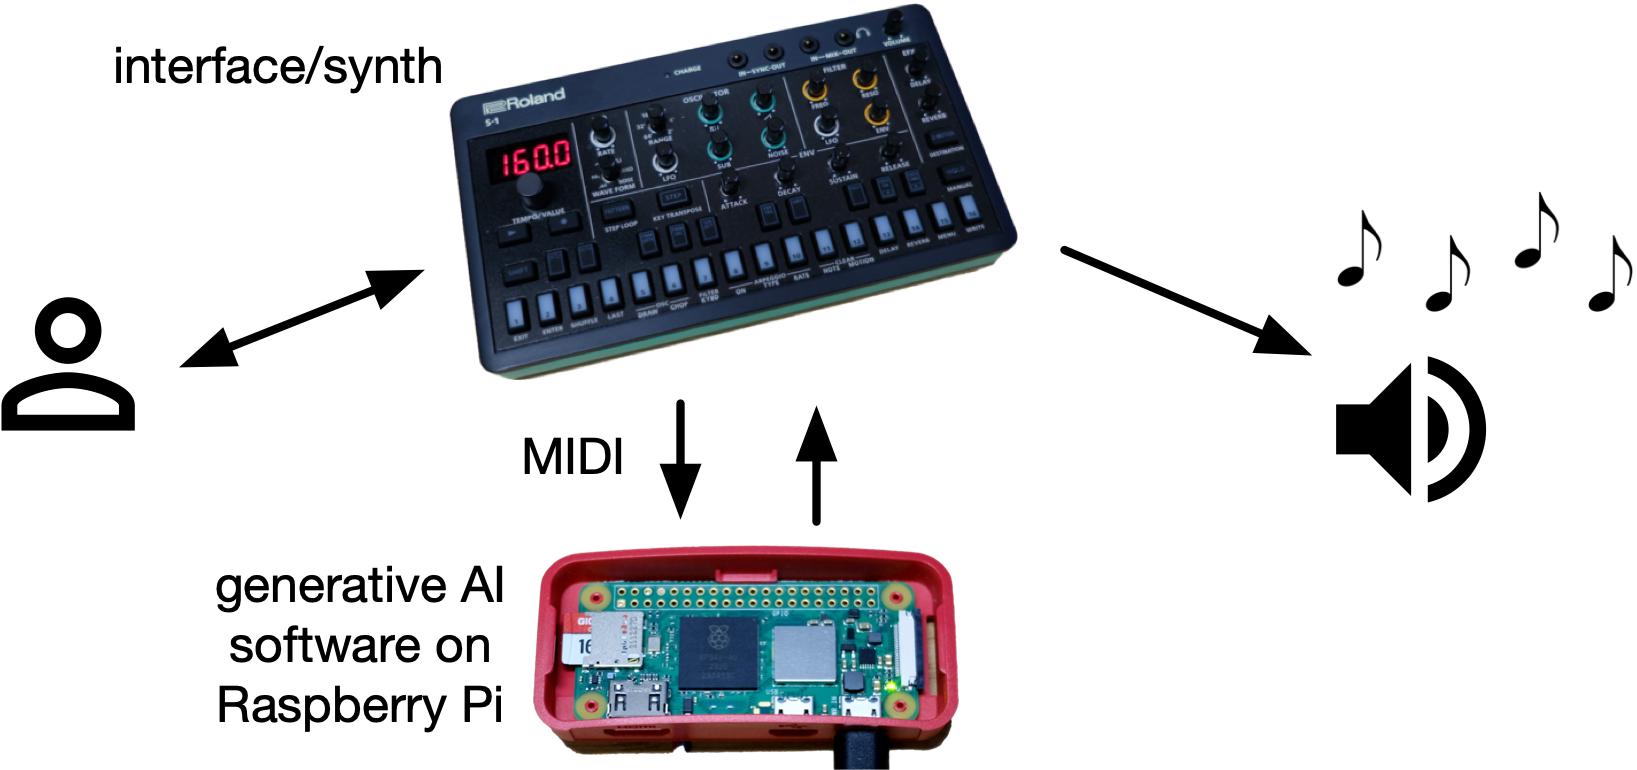
\includegraphics[width=0.5\linewidth]{figures/gen-ai-system-diagram.png}
    \caption{Our generative AI interactive music system with a hardware synthesiser. 
    Our system connects to other devices via MIDI and receives signals from a human performer or can send signals to control sound on the synthesiser. 
    Our software is pre-installed on a Raspberry Pi operating system image for  and runs on even the cheapest Raspberry Pi Zero 2 W (15USD).}
    \label{fig:system-diagram}
\end{figure}

\subsection{Hardware}

Our system uses the Raspberry Pi family of single board computers which are widely available and familiar for many electronic instrument designers. 
Our software works on all Raspberry Pi models that support the 64-bit Raspberry Pi OS which ensures good compatibility with machine learning libraries for Python. 
This includes the inexpensive Raspberry Pi Zero 2 W (15USD as of 2025) that includes a quad-core 64-bit ARM Cortex-A53 at 1GHz with 512MB of RAM and which is small enough (65mm x 30mm) to be incorporated inside new instrument designs.

We have explored several methods of communicating with other devices from the Raspberry Pi. 
MIDI is used as the primary communication format and our software can send MIDI messages via either a USB-connected MIDI interface, a direct USB MIDI connection to a hardware synthesiser, or from the Raspberry Pi's serial (UART) output. 
Our software can also communicate over a network using OSC (open sound control) or WebSockets messages. 
The smallest Raspberry Pi Zero models only support one USB host connection while larger models (e.g., Rasberry Pi 4 Model B) have multiple USB host ports and an Ethernet interface so could support multiple communications channels simultaneously.
For MIDI-over-serial connections, the MIDI connector can be soldered to the GPIO pads corresponding to the Pi's serial (UART) output. 
Providing a MIDI output from the Pi's 3.3V signals is straightforward requiring only two resistors~\cite{MIDI-Manufacturers-Association:2014aa}: 10$\Omega$ between the UART TX pin and pin 5 on the MIDI connector and 33$\Omega$ between the 3.3V output and MIDI pin 4. 
MIDI pin 2 is connected to ground. 
In the setup shown in Figure \ref{fig:self-playing-volca}, the resistors are concealed within the MIDI connector.

\subsection{AI model}

Following Martin and Torresen~\cite{Martin2019}, we use a mixture density recurrent neural network (MDRNN) as the machine learning paradigm for generating a stream of musical data and we apply the Keras-MDN-Layer library~\cite{keras-mdn-layer} to construct this neural network.
Our system uses an MDRNN that generates tuples of data that we interpret as number of musical values and a time delta for when that value should occur in the future. 
The number of musical values is configurable within our software but is at a minimum one, i.e., the system models one musical parameter over time. 
We have experimented with up to 16 parameters modelled simultaneously.
The neural network is autoregressive, so takes the preceding value as input to the generate next, but it is also recurrent, so it stores a lossy history of generated values using LSTM units. 
We typically use small MDRNN models, e.g., 2 layers of 64 LSTM units.
Although this is a very small number of parameters compared to typical generative AI and large language models, it is sufficient for generating musically useful data in real-time on small hardware.
Full evaluation of this AI model is beyond the scope of this paper, but we have benchmarked the inference speed. Our experiments showed that with the small models we use (2-layer LSTM with up to 256 units) individual inference steps are completed in under 5ms on all compatible Raspberry Pi models (Zero 2 W, 3 Model B, 4 Model B) and well under 1ms on the Raspberry Pi 5. These inference speeds are sufficient for representing smooth MIDI signals. 
The time for training a new model depends on the size of the training data and speed of the training computer, but effective models can be trained in under 30 minutes on a normal laptop.

\subsection{Software}

Our system's software is a Python program running on the Raspberry Pi that generates musical data and sends it to external electronic musical instruments.
This program listens to MIDI signals from the instrument and responds with AI-generated continuations of the performance state.
MIDI note-on as well as control change messages are supported so our system is able to play notes as well as change the timbre of a connected instrument.
As mentioned above, our AI model is capable of listening and responding to a number of channels of such MIDI data simultaneously.
Our software records all data that is received from the MIDI interface and stores this as timestamped logs. This means that performing with our system builds up new datasets allowing new AI models to be trained.

An initial configuration is required to choose the MIDI interface and the specific MIDI signals listen and send to. 
Configuring such interaction mappings is a design task that fundamentally changes how a created intelligent musical instrument will function. 
For example, it may be interesting only assign timbral changes to the generative AI system while a performer controls notes (or vice-versa). Alternatively, the performer's notes can be cross-mapped to influence the timbral parameters changed by the generative AI system.
A simple web interface is provided for adjusting the configuration file, downloading logged data of previous performances and uploading new AI models.

The software for our system can be installed using Poetry or Python's pip tool but this can be a laborious process for new users. 
To accelerate setup with a new instrument we pre-install our software on a Raspberry Pi OS image that can be flashed to an SD card. 
The generative AI interaction system and web server programs are started on boot and Ethernet-over-USB is enabled so that the Raspberry Pi can be directly connected to a computer for configuration.


\section{Performance Experiences}\label{case-studies}


This section describes five new intelligent musical instruments and the experience of using them in performance over a period of approximately two years (2024-2025).
In this autobiographical artistic research, these instruments were developed for the first authors' use and tested in live performances, recordings, and demonstrations to expand knowledge about the design space for intelligent musical instruments. The performance style was free improvised music. 
These performance experiences include solo recordings and concerts as well as applying intelligent instruments within ensembles of acoustic and electronic instruments. The following sections introduce the systems in roughly chronological order, including reflections on how the designs could be used in performance and what revisions were made to the AI system in response. These reflections cover the 16 performances, recordings, and demonstrations listed in Table~\ref{tab:perf-corpus}.

\subsection{The Self-Playing Volca}

\begin{figure}
    \centering
    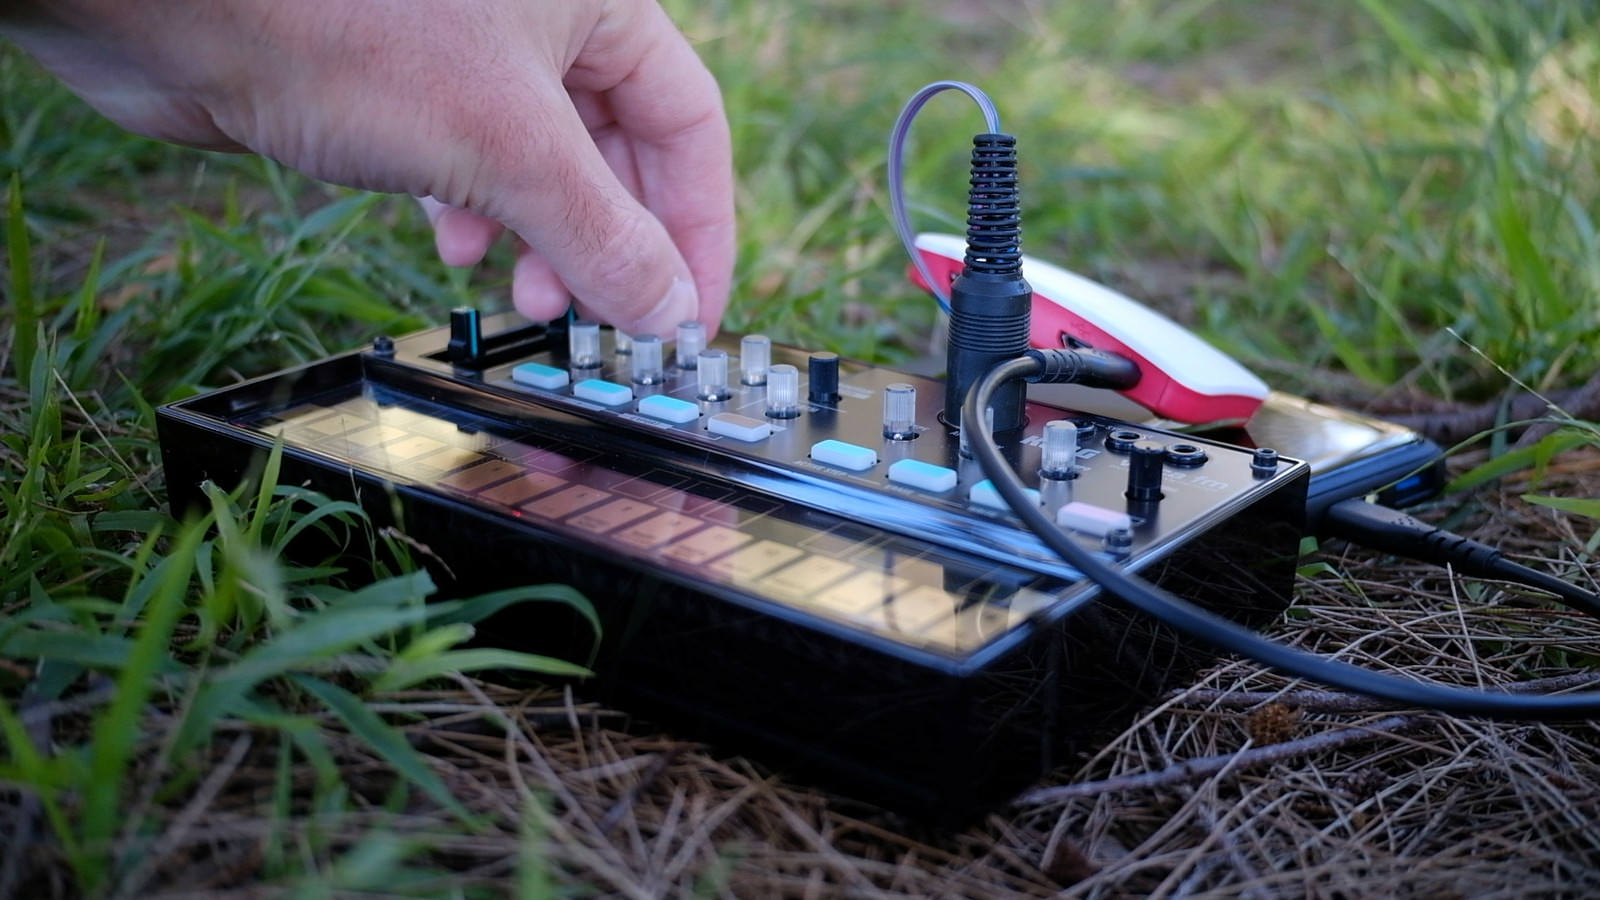
\includegraphics[width=0.5\linewidth]{figures/outside-1.jpg}
    \caption{Battery-powered human-AI interaction on a Korg Volca FM. The generative AI system running on the Raspberry Pi Zero controls pitch and rhythm via the MIDI connector while the musician edits the synth patch. 
    % Video: \url{https://vimeo.com/911078203}
    }
    \label{fig:self-playing-volca}
\end{figure}

The self-playing Volca was a proof-of-concept to establish whether real-time generative-AI MIDI signals from the Raspberry Pi Zero was feasible and musically interesting.
MIDI output was obtained from the Raspberry Pi's GPIO header UART pins and connected to the battery-powered Volca FM.
The AI model was trained on a corpus of around one hour of musical human interaction with a single continuous controller. 
The AI model output (0.0--1.0) was converted to a MIDI pitch value from 0--127 and a corresponding MIDI note-on message scheduled to be sent at the time-delta generated, so the model could control pitch and rhythm on the Volca.

This initial experiment emphasised portability with a completely self-contained and battery-powered system; the Volca FM even has an internal speaker.
The generative AI system played notes while the human performer could adjust the synthesiser's timbre or play overlapping notes on the keyboard; however, the AI model couldn't respond to the performer as the Volca FM has no MIDI output.
This meant that although this experiment started to explore different roles for the human and AI system in controlling the synth, the interaction was necessarily one way. 
The AI model, trained on expressive interaction with a continuous controller, tended to perform glissandi of various speeds, starting points and lengths on the Volca.
These sounded somewhat unusual as the synthesiser re-triggered its envelope for each note.
Performance experiments suggested that this AI model may be more applicable to synthesis parameter control tasks where a musician would like a particular value to change smoothly in an expressive way.

\subsection{The Intelligent MicroFreak and S-1}

\begin{figure}
	\centering
	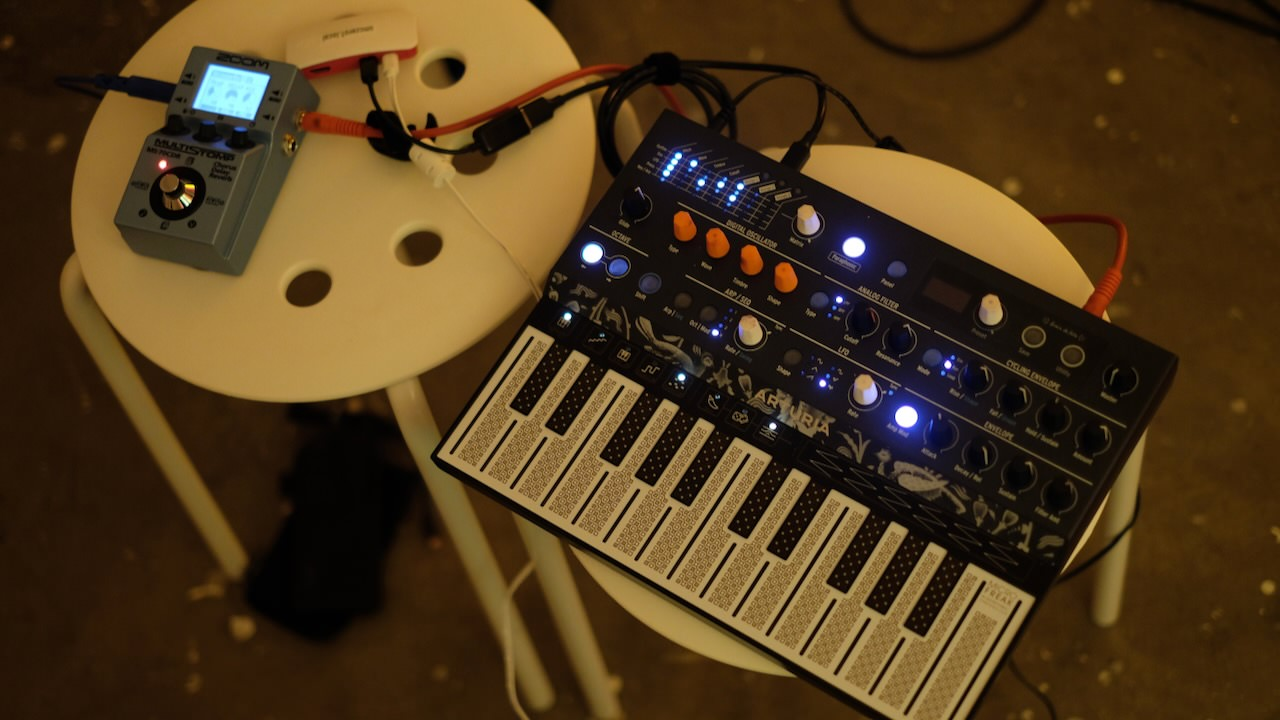
\includegraphics[width=0.49\linewidth]{figures/intelligent-microfreak-169.jpg}
    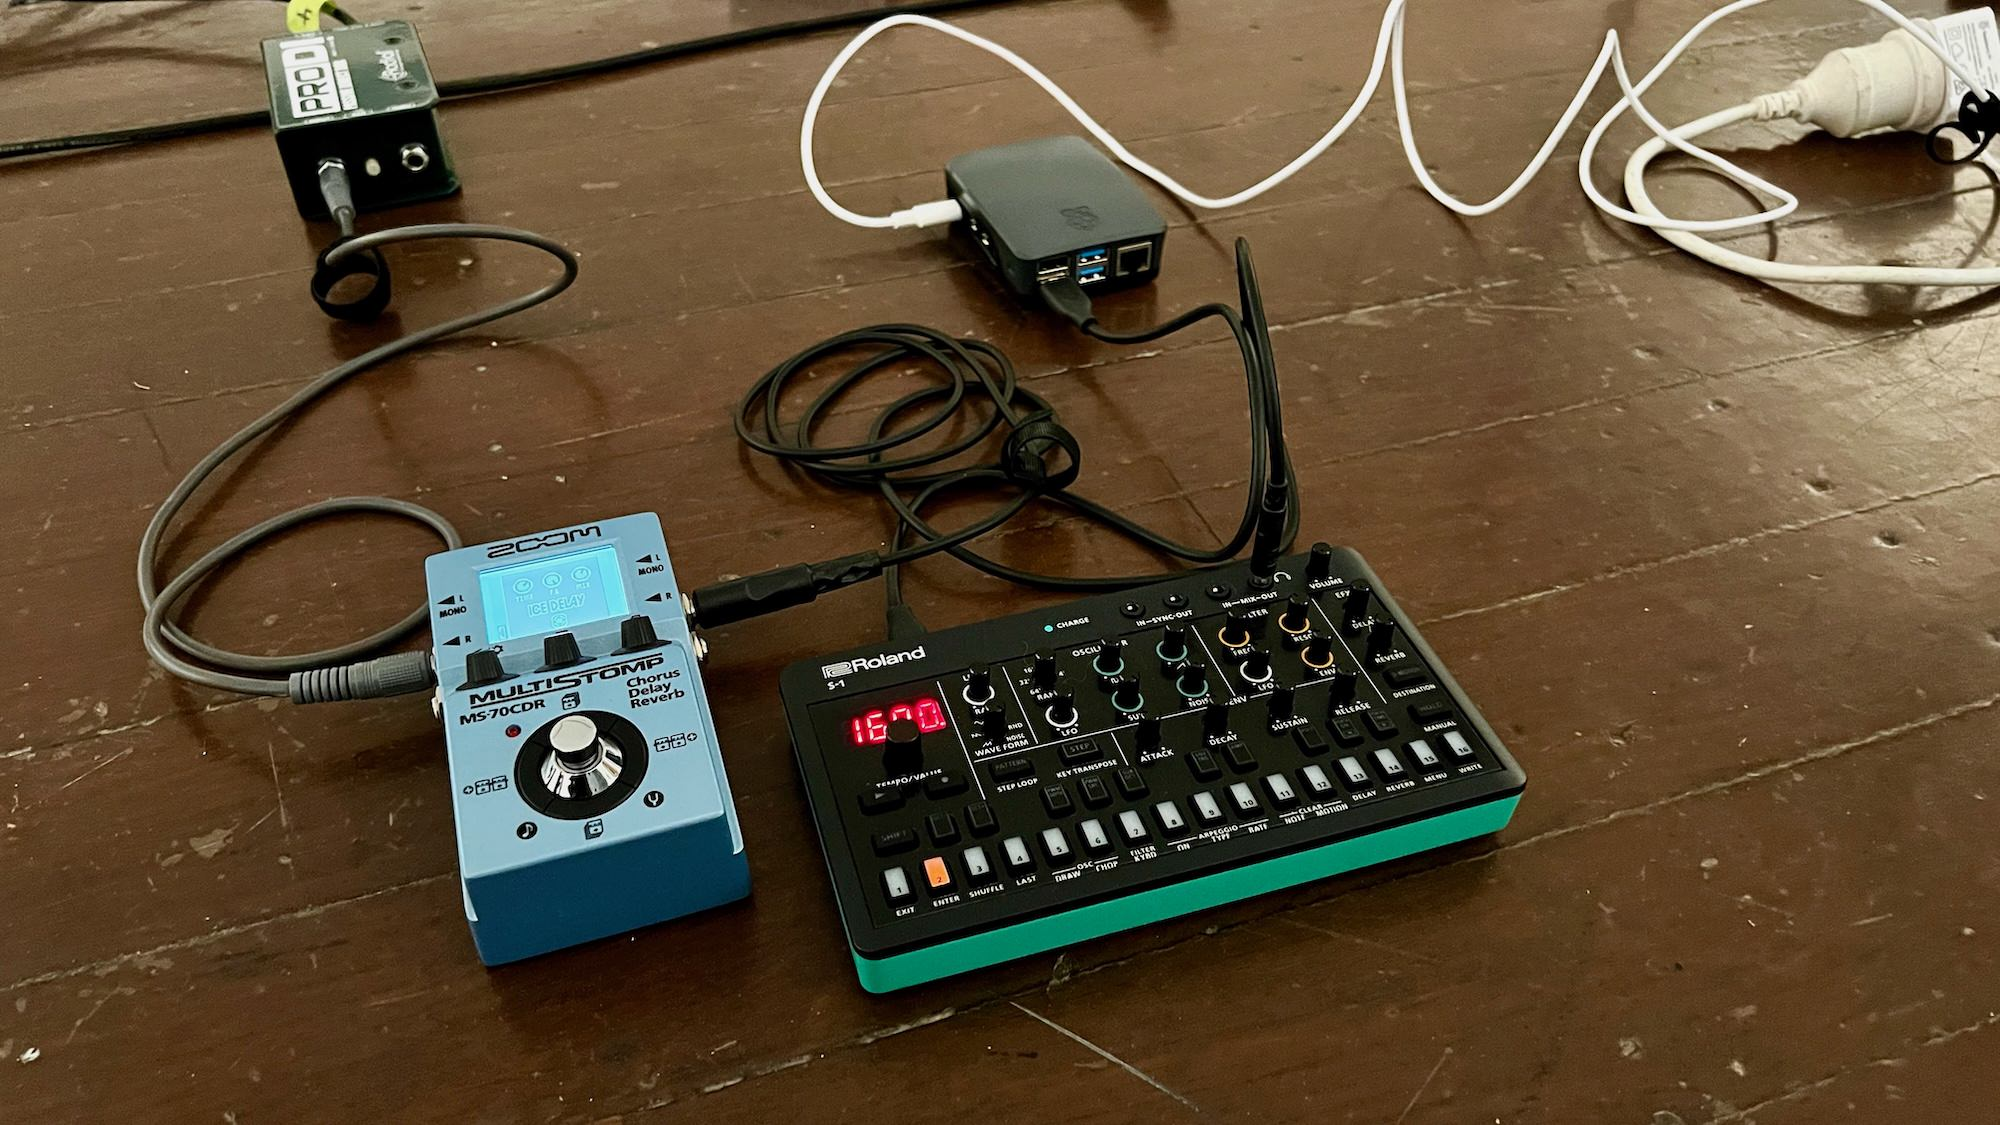
\includegraphics[width=0.49\linewidth]{figures/intelligent-s-1.jpg}
	\caption{Stage setups with a Arturia MicroFreak synthesiser (left) and Roland S-1 (right).
    Our software ran on a Raspberry Pi Zero 2 W (left) or Raspberry Pi 4 (right) and in both cases a Zoom effects pedal provided additional audio effects.
    For both setups, the generative AI system generated note data (tracking the keyboard) and seven timbral parameters (tracking knobs on the synthesiser interface).}
	\label{fig:intelligent-synth}
\end{figure}

Hardware synths with MIDI outputs and inputs promised to support two-way interaction with our system.
The capacity for MIDI-over-USB connections was developed to enable our system to connect directly to synthesisers with built-in USB-MIDI interfaces where notes from their keyboard and control changes from their knobs and other interface elements can be sent and received over MIDI.
In many cases, simultaneous control of the synthesiser from the hardware interface and from MIDI signals is possible allowing shared human-AI interaction. 
In our case, the AI system responded in a call-and-response manner so that when the performer adjusted the synth controls and played notes, the AI system tracked these signals. When the human stopped for a certain amount of time the AI system took over the controls.

We first used an Arturia MicroFreak synthesiser with the generative AI system controlling eight parameters: note-on messages, and seven timbral parameters available to the performer via knobs on the synthesiser face.
This system was used in individual and group improvisations with performers on a variety of other instruments.
The system was portable (see Figure \ref{fig:intelligent-synth}) with the tiny Raspberry Pi Zero and an effect pedal accompanying the small synthesiser.
This AI model was trained on data sourced from the first author's improvisation on eight continuous controllers.
In performance, the AI model produced musically satisfying material.
Unlike a human, the AI system is able to adjust many parameters simultaneously, resulting in an inhuman but exciting exploration of the synth parameter space.
In non-AI performances, the author would primarily play notes on the synthesiser with occasional timbral changes; however, the AI interactions update the timbral parameters in between phrases and in some cases in between notes, leading to varying and unique sounds. 
To enhance this effect, the call-and-response switch-over time was set to 0.1 seconds.

This performance concept was further explored with a Roland S-1 synthesiser where a similar mix of note and parameters signals were controlled by the AI system.
The very small size of this synth compromises the playability of the keyboard but using the AI system led to less reliance on the keys. In performance, more focus could be put on timbral parameter setting, allowing the AI system to improvise notes in between human-selected parameter changes which were also under the control of the AI model leading to surprising timbral outcomes.

\subsection{The Intelligent Digital Audio Workstation}

\begin{figure}
    \centering
    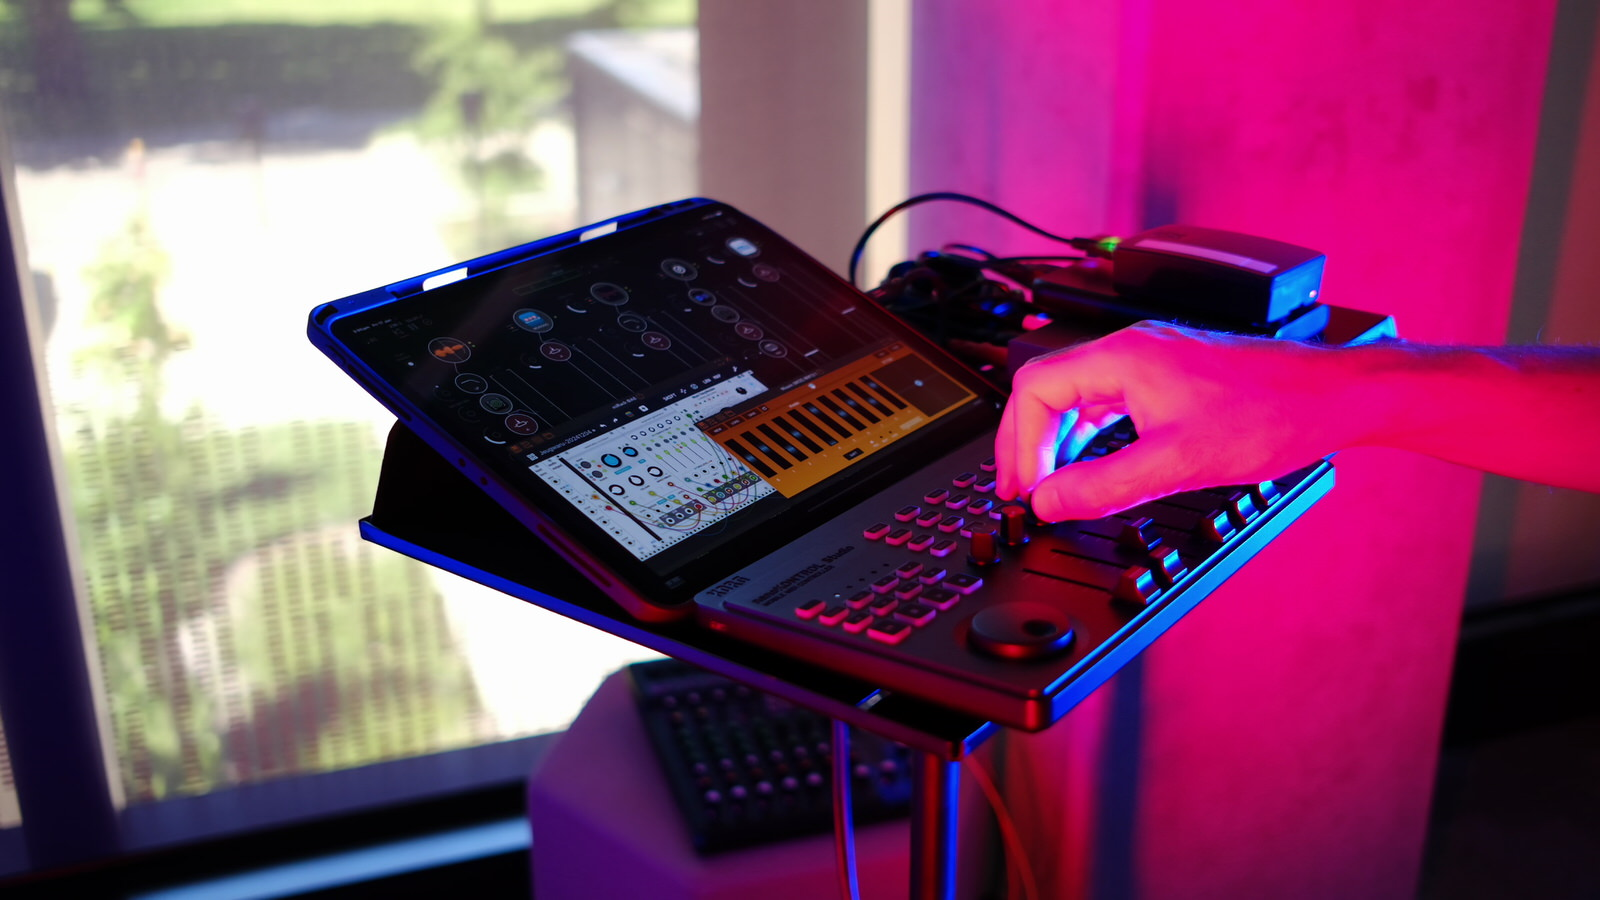
\includegraphics[width=0.5\linewidth]{figures/ipad-perf-2.jpg}
    \caption{Software synthesisers used in an intelligent instrument setup. Digital audio workstation (DAW) software ran on the iPad which is connected via MIDI to our generative AI system on a Raspberry Pi 4. The performer can interact with the instrument using the iPad touchscreen or a hardware controller interface.}
    \label{fig:intelligent-daw}
\end{figure}

Much contemporary electronic music is performed on software synthesisers and audio files loaded into digital audio workstation (DAW) software~\cite{daws-reuter-2021, Clauhs:2023aa}.
DAW software supports MIDI input and output to control parameters with internal routing and mapping possibilities.
We experimented with connecting our system to a DAW running on a computer or tablet via an inexpensive USB MIDI interface.
This represents a convenient way to design new intelligent musical instruments and interactions as both the DAW and our generative AI system are highly configurable.

An example is illustrated in Figure \ref{fig:intelligent-daw} where a DAW and software plugin host, Kymatica AUM (Audio Mixer), ran on an iPad with eight different sound generators available in channel strips with associated effects.
The sound generators were a mix of software synthesisers and audio file players.
Our generative AI system was configured to respond to eight different MIDI control change channels and generate four different channels of MIDI notes and four channels of control change data.
This input and output data is routed internally in AUM and assigned to control different parameters and notes within the sound generators.
The performer could influence the AI generated data on the iPad touchscreen via a software MIDI controller or with a hardware MIDI controller connected to AUM with Bluetooth.
This setup is highly flexible in that different sound generators can be loaded or unloaded and the MIDI routing can be adjusted for different performance requirements without necessarily reconfiguring the generative AI software on the Raspberry Pi.

The ability to map generative AI signals over a simple MIDI connection is an advantage for performing with tablets or laptops where a installing a Python AI application is either impossible or inconvenient.
This specific setup has been used in solo and ensemble electronic music improvisations.
The ability to re-map MIDI signals from the generative AI system to any parameter in the software synths was a way to evolve the intelligent instrument without retraining or modifying the generative AI system. 
Signals were mapped to areas where they were musically useful and software synths were swapped out with others or adjusted to sound significantly different. 
Having multiple synths loaded in a DAW allowed the output sound to be mixed and adjusted leading to quite different musical characteristics in between performances. 
While all parameters could be adjusted within the touchscreen interface, the addition of the hardware MIDI controller with physical knobs for influencing the generative AI system was an effective way to keep track of the autonomous components of the instrument.

\subsection{Intelligent Setups}

Talk about combining multiple inputs and outputs.

% Please add the following required packages to your document preamble:
% \usepackage{booktabs}
\begin{table}[]
\caption{Configuration of the performances, recordings, and demonstrations considered as part of the first-person artistic research process in this work throughout 2024 and 2025. This list does not include rehearsal or practice sessions that also took place.
A "*" in the configuration column denotes where more than one performer used an intelligent instrument studied in this paper, other duo and group performances involved one intelligent instrument (performed by the first author) with other performers using acoustic and conventional electronic instruments.}
\label{tab:perf-corpus}
\begin{tabular}{@{}llll@{}}
Date           & Type           & Configuration & Intelligent Instrument      \\ \midrule
February 2024  & Recording      & Solo          & Volca                       \\
May 2024       & Recording      & Solo          & Microfreak                  \\
May 2024       & Performance    & Group*        & Microfreak, DAW (AUM, Live) \\
June 2024      & Performance    & Duo           & Microfreak                  \\
June 2024      & Performance    & Group         & Microfreak                  \\
September 2024 & Demonstration  & Solo          & S-1                         \\
September 2024 & Performance    & Solo          & Microfreak, S-1             \\
September 2024 & Performance    & Duo           & Microfreak                  \\
October 2024   & Performance    & Group         & S-1                         \\
December 2024  & Recording      & Duo*          & DAW (AUM, Live)             \\
January 2025   & Recording      & Solo          & S-1, DAW                    \\
August 2025    & Performance    & Group         & S-1, DAW                    \\
October 2025   & Demonstration & Solo          & S-1, Microfreak             \\
November 2025  & Performance    & Duo           & Setup (S-1/xTouch)          \\
November 2025  & Performance    & Duo           & Setup (S-1/QuNeo)           \\
December 2025  & Recording      & Duo           & Setup (S-1/QuNeo)           \\
\end{tabular}
\end{table}



\section{Discussion}

\subsection{Limitations}


\section{Conclusions}\label{conclusions}

This paper has presented our generative AI system for live music performance as a tool for designing and experimenting with new intelligent musical instruments. 
We argue that the design space for intelligent musical instruments using present AI techniques has yet to be explored and that small-data approaches, such as our system, can lead to artist-centred musical AI.
Experiments using our system with hardware synths and software DAWs have demonstrated that it is feasible, flexible and musically useful.
In the hardware synth examples, AI-control over notes and timbral parameters led to unique performances and sounds, making up for limitations in synth interface design.
Our intelligent DAW demonstrated the flexibility of our system when coupled with highly configurable DAW MIDI mappings and expanding the design possibilities for interactions with a DAW as an instrument.
This work contributes design possibilities explored in one creative practice with this system through a first-person reflective process to the ongoing conversation within HCI about how generative AI might be applied in interactive systems.
Future work could examine the impact of updating models over time with artist-sourced data, and engage artists in co-design processes for creating new intelligent musical instruments.

%% The Ethical Standards section is mandatory for all NIME submissions.
\section{Ethical Standards}

This paper involved autobiographical study of new interfaces from the author's perspective.
Where performances were in group settings, other group members were creative collaborators rather than research participants and have been acknowledged below.

\begin{acks}
My thanks to collaborators and creative partners who made music with me as part of this project: Alec Hunter, Yichen Wang, Sandy Ma, Richard Johnson and the SoundOut Collective. 
\end{acks}

\bibliographystyle{ACM-Reference-Format}
\bibliography{references} 

\end{document}

% Our system has been tested in the context of electronic music improvisation where control over a synthesiser is shared between a human and the GenAI MIDI Plug. Figure \ref{fig:human-ai} and our accompanying video\footnote{\url{https://vimeo.com/911078203}} shows excerpts from an outdoor battery-powered improvisation. In this example, the synthesiser is a Korg Volca FM with note values (pitch and rhythm) controlled by the GenAI MIDI Plug. The musician adjusts parameters on the synthesiser patch including pitch shifting the GenAI MIDI signals by octaves.

% The experience so far with this system is positive. The signal from the GenAI MIDI Plug can be contextualised as a more expressive and unpredictable kind of LFO (low frequency oscillator) within a synth setup. As it's modelled on human-sourced data, it noodles, pauses, explores different parts of the output range, stops completely sometimes and starts up again at (perhaps) annoying moments. Although it exhibits some behaviours that could be programmed into a hard-coded signal generator it also has a level of stochasticity and variation that that would be more complicated to construct heuristically. Importantly, the very small size of the system means that it can fit into battery-powered electronic music setups. The price of the system means that potentially more than one could be affordably applied in any one performance.

% The intention of this research has been not just to create one GenAI MIDI Plug but to demonstrate the feasibility of this approach to instrument designers who may wish to adapt this idea.
% The hardware aspects of our system demonstrate a really simple way of connecting a Raspberry Pi Zero to existing electronic music systems. 
% Although the software is effective, the Keras MDN Layer~\cite{keras-mdn-layer} library presently requires the full Tensorflow and TensorFlow-Probability libraries. 
% The newer 64-bit Raspberry Pi OS should make it easier to install these, but in our experience we were still using a custom build of Tensorflow\footnote{\url{https://github.com/PINTO0309/Tensorflow-bin}} for the Raspberry Pi which may be intimidating for beginners to install. 
% Once the system is running, data generation with the MDRNN is quick; however, the process of booting, loading Tensorflow, and starting generation takes around 90 seconds. 
% There may be potential to port this system to use lighter libraries (e.g., Tensorflow-Lite) that may load more quickly from boot and could also improve the installation experience for instrument designers.

% This work has introduced a minimal approach to creating an intelligent musical instrument, the GenAI MIDI Plug. This research aims to address gaps in creative practice and interaction that have been identified in NIME applications of generative AI. While enabling artist-led data collection and training may support a small-data approach, cheap minimal battery-powered AI music controllers could encourage a greater range of experimentation and prototyping among the wider music community.



% \begin{figure}
%     \centering
%     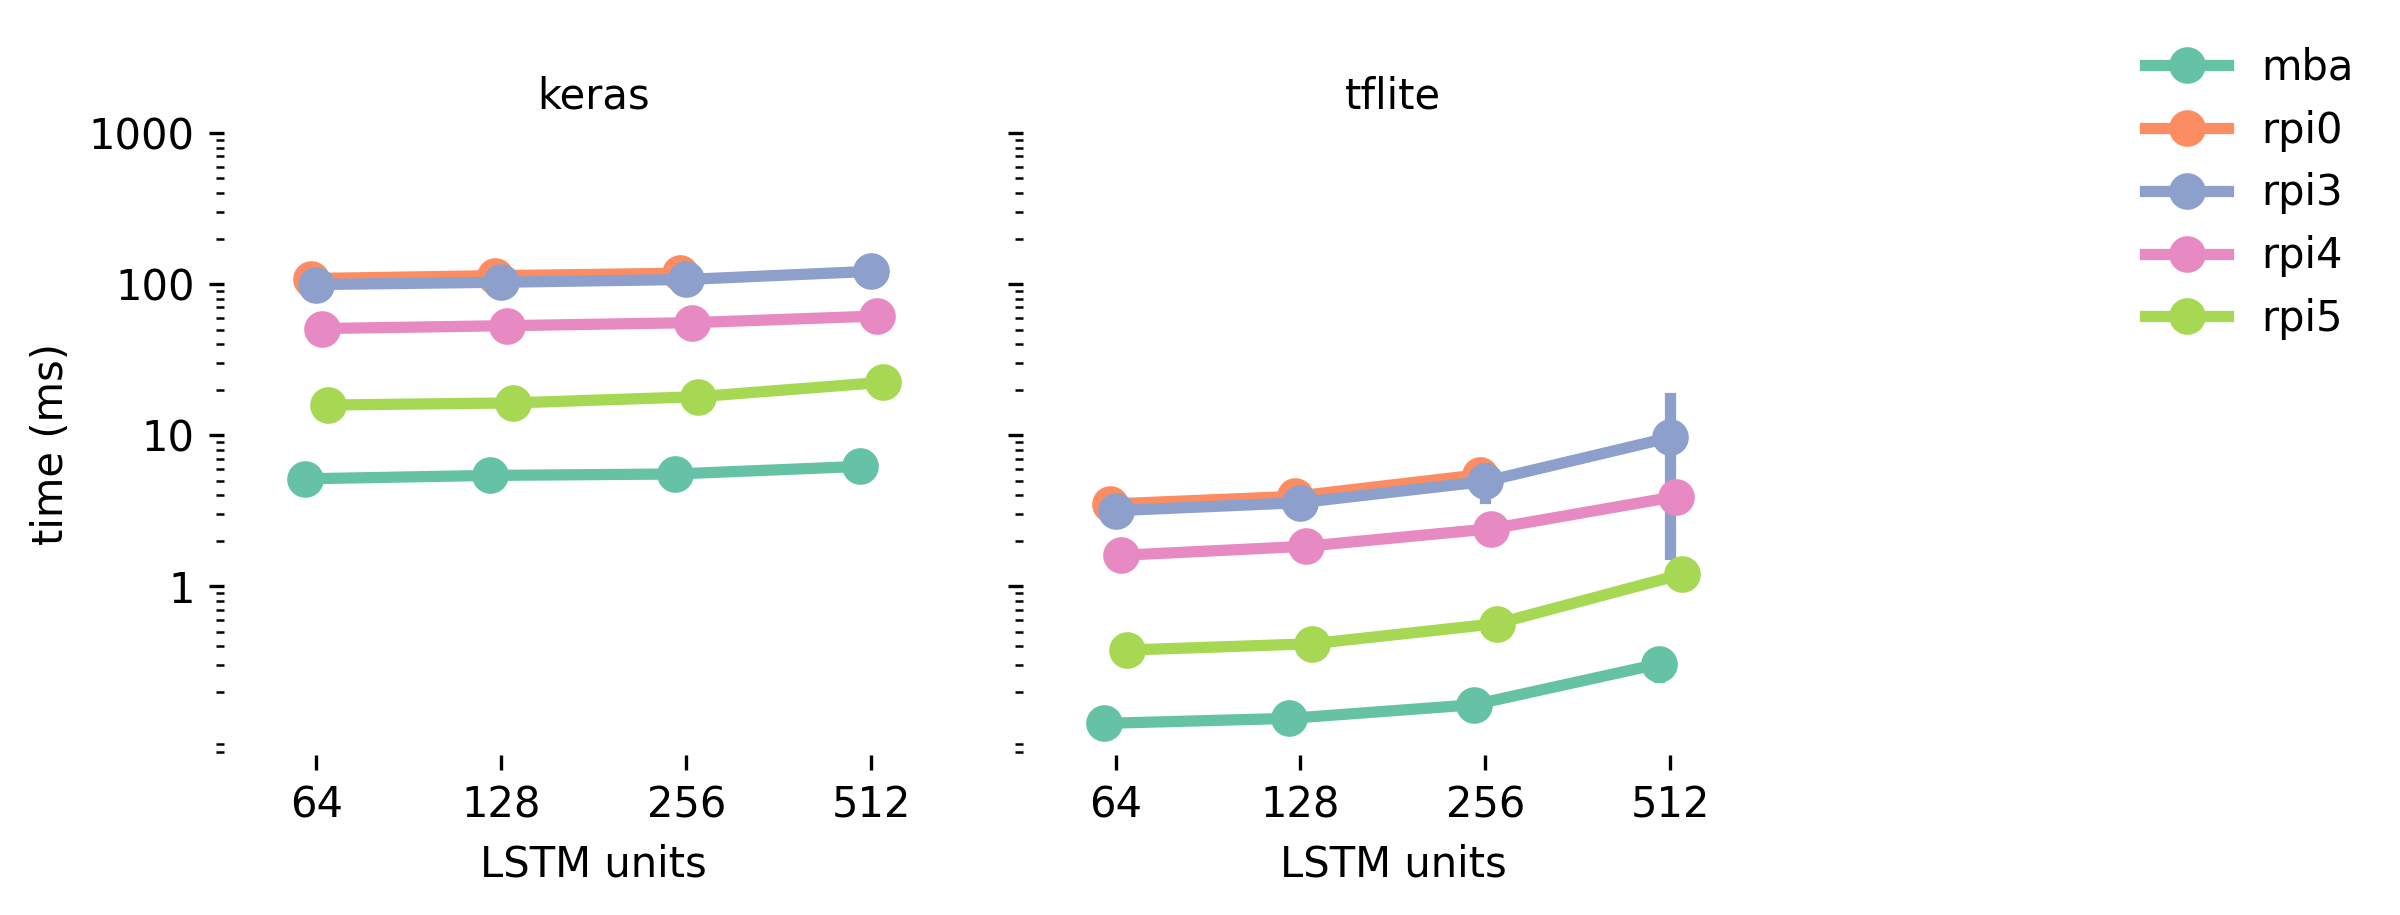
\includegraphics[width=0.99\linewidth]{figures/prediction_time_against_units_facet_log.png}
%     \caption{A plot of the time for single AI predictions on different hardware and model size. Even the slowest Raspberry Pi Zero 2 W runs predictions under 5ms using Tensorflow Lite.}
%     \label{fig:inference-time}
% \end{figure}

% Our generative AI system includes an implementation of a mixture density recurrent neural network (MDRNN), appropriate for generating expressive musical signals from small artist-centered datasets. 
% This system can communicate to existing software and hardware musical systems using MIDI over USB, standard MIDI hardware connections, as well as OSC or WebSockets over a network.
% In this way, existing musical systems can be integrated with a generative AI system to create an intelligent musical instrument that can play by itself or take turns with and adapt to a human performer's input.
% In this research we introduce our generative AI system and explore its potential through a series of instrument designs and artistic research performances.
% Our experiments show that this idea is feasible and useful for experimenting with human-AI musical interaction.
% We distill lessons learned through ideation, development and performance with these systems to propose design recommendations for future intelligent musical instruments.
% This work could serve as a basis for prototyping further intelligent musical instruments and exploring their application in different creative practices.

% \begin{figure}
%     \centering
%     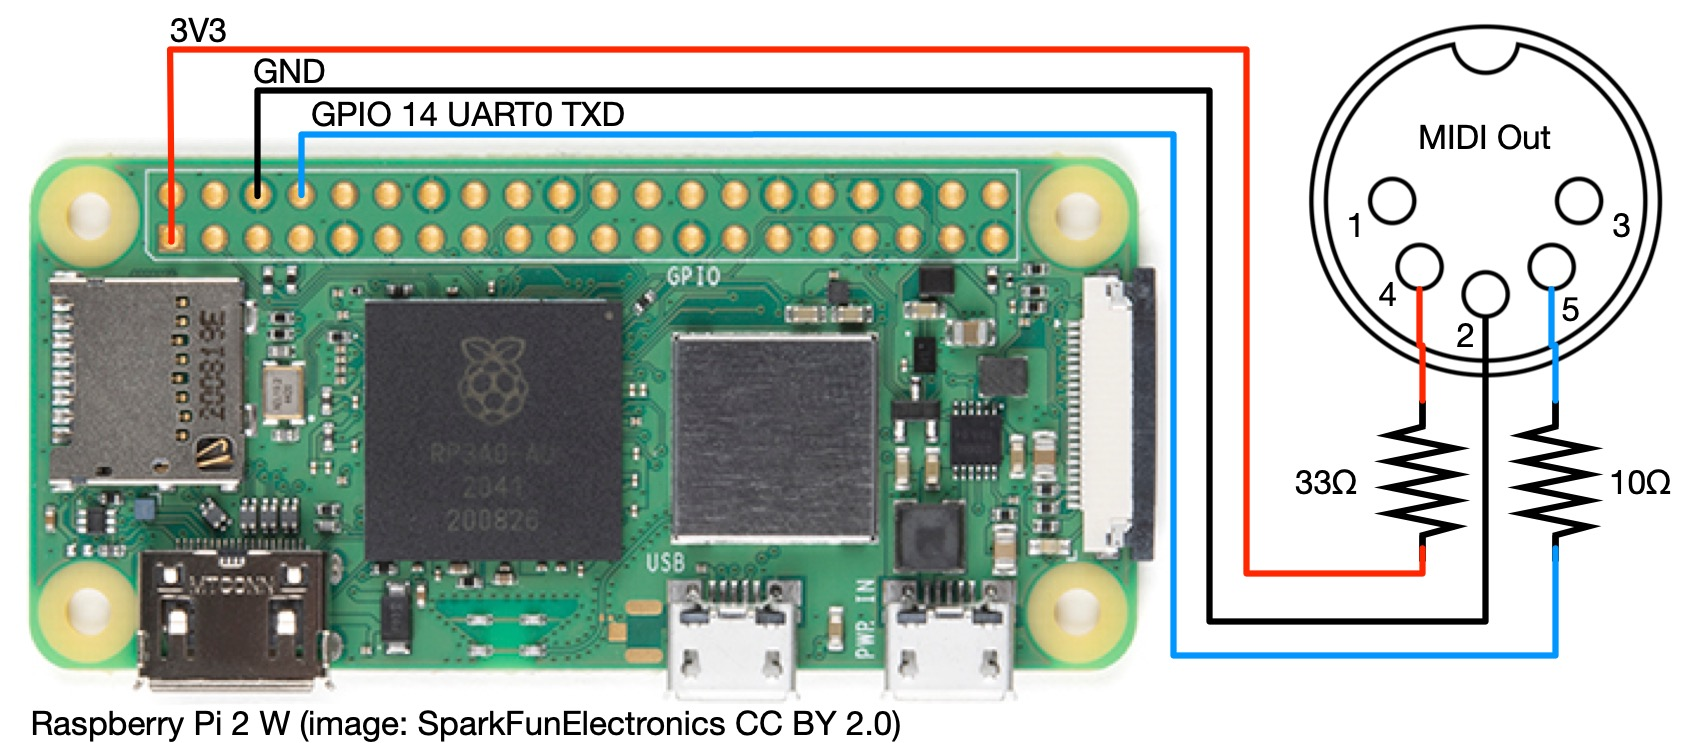
\includegraphics[width=\columnwidth]{figures/sf-image.jpg}
%     \caption{Circuit diagram for the GenAI MIDI Plug. A MIDI output can be obtained from a Raspberry Pi with the addition of only two resistors that can be concealed inside the MIDI connector.}
%     \label{fig:enter-label}
% \end{figure}

% \begin{figure}
%     \centering
%     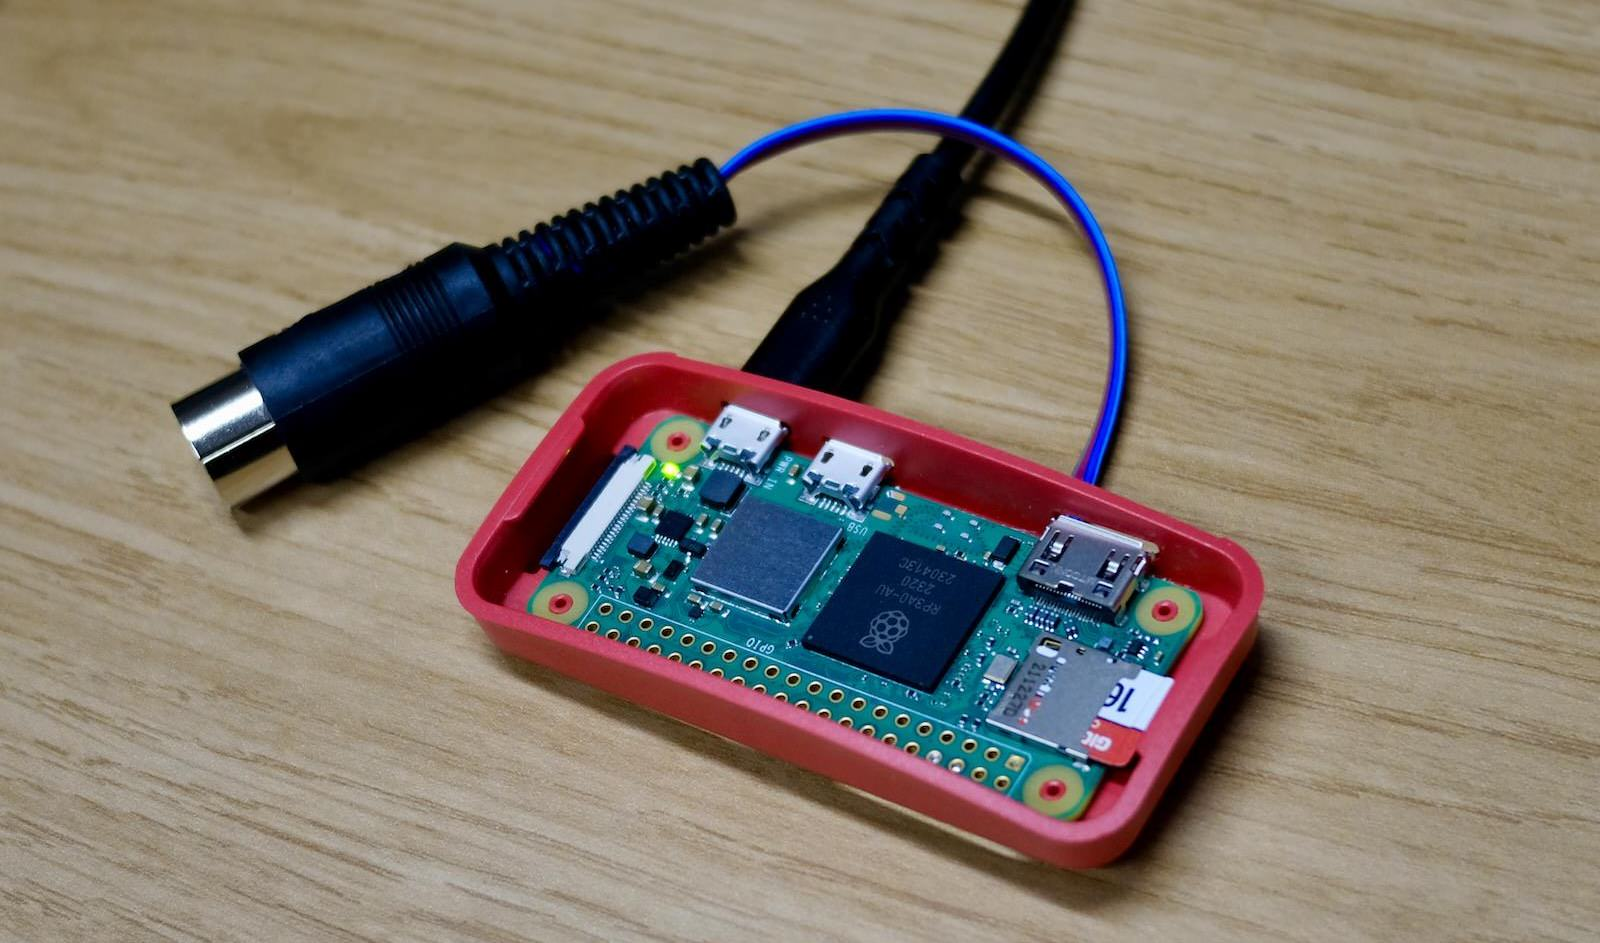
\includegraphics[width=0.8\linewidth]{figures/desk-angle.jpg}
%     \caption{The GenAI MIDI Plug with cover removed. The hardware consists of a Raspberry Pi Zero 2 W with case, 16GB microSD card, and a MIDI connector soldered directly to the Raspberry Pi.}
%     \label{fig:system-photo}
% \end{figure}
